\documentclass[tikz, border=3mm]{standalone}
\usepackage{tikz}
\usetikzlibrary{arrows.meta, calc}

\begin{document}
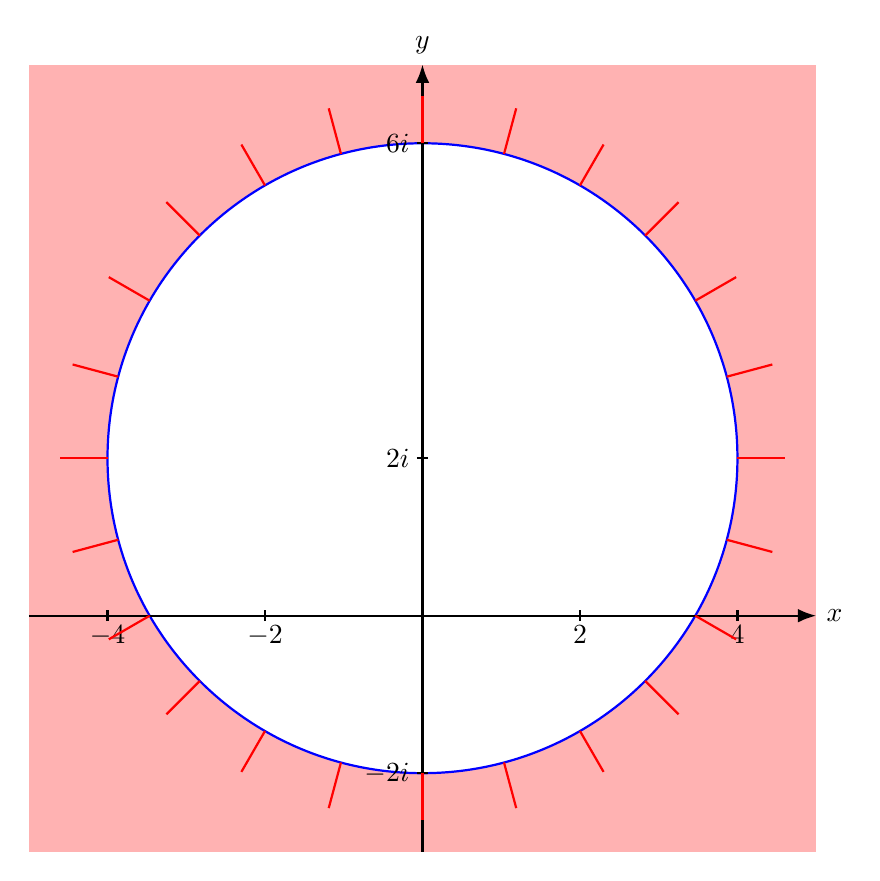
\begin{tikzpicture}[
    >=Latex, % Set default arrow tip style
    labelstyle/.style={inner sep=2pt}, % Style for the labels
    tick/.style={thick} % Style for tick marks
]

    % Define center and radius based on labels
    \coordinate (center) at (0, 2);
    \def\radius{4} % Distance from (0,2) to (0,6) or (0,-2)
    \def\axlim{5} % Axis limit (used for fill area too)
    \def\axymin{-3} % Min y axis limit
    \def\axymax{7}  % Max y axis limit
        \def\outerradius{\radius + 0.6} % How far rays extend (increased slightly)


    % --- Layer 1: Red Shaded Background ---
    % Fill a rectangle covering the view area with a light red
    \fill[red!30] (-\axlim, \axymin) rectangle (\axlim, \axymax);

    % --- Layer 2: White Fill to Erase Inside Circle ---
    % Fill the circle area with white (or background color)
    \fill[white] (center) circle (\radius);

    % --- Layer 3: Blue Circle Border ---
    % Draw the blue circle border on top of the fills
    \draw[blue, thick] (center) circle (\radius);

    % --- Layer 4: Axes and Ticks (Draw last to be on top) ---
    % Axes
    \draw[->, thick] (-\axlim, 0) -- (\axlim, 0) node[right] {$x$};
    \draw[->, thick] (0, \axymin) -- (0, \axymax) node[above] {$y$};

    % X-axis Ticks (example values)
    \foreach \x in {-4, -2, 2, 4} {
        \draw[tick] (\x, -2pt) -- (\x, 2pt) node[below=2pt] {$\x$};
    }
    % Y-axis Ticks (key values)
    \foreach \y/\label in {-2/{-2i}, 2/{2i}, 6/{6i}} {
        \draw[tick] (-2pt, \y) -- (2pt, \y) node[left=3pt] {$\label$};
    }
    % Add tick for origin if desired
    % \node[below left=1pt] at (0,0) {$0$};

\foreach \angle in {0, 15, ..., 345} { % Decreased step from 30 to 15
        % Draw slightly curved lines radiating outwards from circle boundary
        \draw[red, thick, bend left=5] ($(center)+(\angle:\radius)$) -- ($(center)+(\angle:\outerradius)$);
    }
\end{tikzpicture}
\end{document}